% !TEX root = ./CM_A-Exercicios_Resolucoes.1.tex
\providecommand\mainfilename{"./CM_A-Exercicios_Resolucoes.tex"}
\providecommand \subfilename{}
\renewcommand   \subfilename{"./CM_A-Exercicios_Resolucoes.1.tex"}
\documentclass[\mainfilename]{subfiles}

% \tikzset{external/force remake=true} % - remake all

\begin{document}

\graphicspath{{\subfix{./.build/figures/CM_A-Exercicios_Resolucoes.1}}}
\tikzsetexternalprefix{./.build/figures/CM_A-Exercicios_Resolucoes.1/graphics/}

\mymakesubfile{1}
[CM A]
{Estruturas Cristalinas} % Subfile Title
{Estruturas Cristalinas} % Part Title

\begin{questionBox}1{ % Q1
    Para as estruturas cúbica simples (\emph{CS}), cúbica de corpo centrado (\emph{CCC}) e cúbica de faces centradas (\emph{CFC}), calcule:
} % Q1
    \begin{questionBox}2{ % Q1.1
        A relação entre o parâmetro de rede \emph{a} e o ráio atómico
    } % Q1.1
        \answer{}

        \begin{multicols}{2}
            
            \subsubquestion{CS}
            % \tikzset{external/remake next=true}
            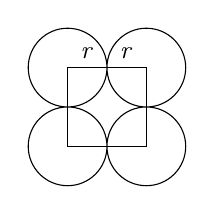
\begin{tikzpicture}
                
                % Square
                \draw[-] (0,0) -- (1,0) -- (1,1) -- (0,1) -- cycle;
                % Circles
                \draw
                (0,0) circle[radius=0.5]
                (1,0) circle[radius=0.5]
                (1,1) circle[radius=0.5]
                (0,1) circle[radius=0.5];
                % radius
                \path (0,1) 
                to node[above, node font={\small}]{\textit{r}} (0.5,1) 
                to node[above, node font={\small}]{\textit{r}} (1,1);
                
            \end{tikzpicture}
            \begin{flalign*}
                &
                    a_{\text{CS}} = 2\,r
                &
            \end{flalign*}
    
            \subsubquestion{CCC}
            % \vspace{-3ex}
            % \tikzset{external/remake next=true}
            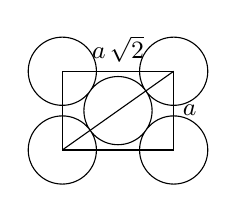
\begin{tikzpicture}
                
                % Square
                \draw[-] (0,0) 
                -- (1.414213562373095,0) 
                -- node[right,node font={\small}]
                {\(a\)}
                (1.414213562373095,1) 
                -- node[above, node font={\small}]
                {\(a\,\sqrt{2}\)}
                (0,1) -- cycle;
                % triangle
                \draw[-] (0,0)
                -- (1.414213562373095,1);
                % Circles
                \draw
                (1.414213562373095,0)   circle[radius=0.433012701892219]
                (1.414213562373095,1)   circle[radius=0.433012701892219]
                (0,1)                   circle[radius=0.433012701892219]
                (0,0)                   circle[radius=0.433012701892219]
                (0.707106781186548,0.5) circle[radius=0.433012701892219];
                % radius
                % \path (0,1) 
                % to node[above, node font={\small}]{\textit{r}} (0.5,1) 
                % to node[above, node font={\small}]{\textit{r}} (1,1);
                
            \end{tikzpicture}
            \begin{flalign*}
                &
                    a_{\text{CCC}}^2 
                    + (a_{\text{CCC}}\,\sqrt{2})^2
                    =(4\,r)^2
                    \implies &\\&
                    \implies
                    a_{\text{CCC}}
                    =4\,r/\sqrt{3}
                &
            \end{flalign*}
    
            \subsubquestion{CFC}
            % \vspace{-3ex}
            % \tikzset{external/remake next=true}
            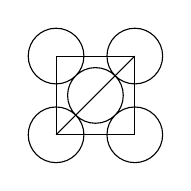
\begin{tikzpicture}
                
                % Square
                \draw[-] (0,0) -- (1,0) -- (1,1) -- (0,1) -- cycle;
                % Triangle
                \draw[-] (0,0) -- (1,1);
                % Circles
                \draw
                (0,0)     circle[radius=0.353553390593274]
                (1,0)     circle[radius=0.353553390593274]
                (0,1)     circle[radius=0.353553390593274]
                (1,1)     circle[radius=0.353553390593274]
                (0.5,0.5) circle[radius=0.353553390593274];
                % radius
                % \path (0,1) 
                % to node[above, node font={\small}]{\textit{r}} (0.5,1) 
                % to node[above, node font={\small}]{\textit{r}} (1,1);
                
            \end{tikzpicture}
            \begin{flalign*}
                &
                    a_{\text{CFC}}
                    =4\,r\,\cos(\pi/4)
                    =2\,r\,\sqrt{2}
                &
            \end{flalign*}
        \end{multicols}
    \end{questionBox}

    \begin{questionBox}2{ % Q1.2
        O número de átomos por célula unitária
    } % Q1.2
        \answer{}
            
        \begin{questionBox}3b{ % Q1.2.1
            CS
        } % Q1.2.1
            % \tikzset{external/remake next=true}
            \begin{tikzpicture}
                
                % Circles 2
                \begin{scope}[shift={(-3,0)}]
                    % Cube
                    \draw[-]
                    (0,0,0)
                    -- (1,0,0)
                    -- (1,1,0)
                    -- (0,1,0)
                    -- (0,0,0)
                       (0,0,1)
                    -- (1,0,1)
                    -- (1,1,1)
                    -- (0,1,1)
                    -- (0,0,1)
                    (0,0,0) -- (0,0,1)
                    (0,1,0) -- (0,1,1)
                    (1,1,0) -- (1,1,1)
                    (1,0,0) -- (1,0,1);
                    % Circles
                    \fill[ball color=Graph33] (0,0,0) circle (.5);
                    \fill[ball color=Graph33] (1,0,0) circle (.5);
                    \fill[ball color=Graph33] (1,1,0) circle (.5);
                    \fill[ball color=Graph33] (0,1,0) circle (.5);
                    % 
                    \fill[ball color=Graph31] (0,0,1) circle (.5);
                    \fill[ball color=Graph31] (1,0,1) circle (.5);
                    \fill[ball color=Graph31] (1,1,1) circle (.5);
                    \fill[ball color=Graph31] (0,1,1) circle (.5);
                \end{scope}

                % Circles 2
                \begin{scope}[shift={(0,0)}]
                    % Cube
                    \draw[-]
                    (0,0,0)
                    -- (1,0,0)
                    -- (1,1,0)
                    -- (0,1,0)
                    -- (0,0,0)
                        (0,0,1)
                    -- (1,0,1)
                    -- (1,1,1)
                    -- (0,1,1)
                    -- (0,0,1)
                    (0,0,0) -- (0,0,1)
                    (0,1,0) -- (0,1,1)
                    (1,1,0) -- (1,1,1)
                    (1,0,0) -- (1,0,1);
                    % Circles
                    \fill[ball color=Graph31] (0,0,1) circle (.5);
                    \fill[ball color=Graph31] (1,0,1) circle (.5);
                    \fill[ball color=Graph31] (1,1,1) circle (.5);
                    \fill[ball color=Graph31] (0,1,1) circle (.5);
                \end{scope}

                \begin{scope}[shift={(3,0)}]
                    % Circles
                    \fill[ball color=Graph33] (0,0,0) circle (.5);
                    \fill[ball color=Graph33] (1,0,0) circle (.5);
                    \fill[ball color=Graph33] (1,1,0) circle (.5);
                    \fill[ball color=Graph33] (0,1,0) circle (.5);
                    % Cube
                    \draw[-]
                    (0,0,1)
                    -- (1,0,1)
                    -- (1,1,1)
                    -- (0,1,1)
                    -- (0,0,1)
                    (0,0,.5) -- (0,0,1)
                    (0,1,.5) -- (0,1,1)
                    (1,1,.5) -- (1,1,1)
                    (1,0,.5) -- (1,0,1);
                \end{scope}
                
            \end{tikzpicture}
            \begin{flalign*}
                &
                    n_{CS} = 8*1/8 = 1
                &
            \end{flalign*}
        \end{questionBox}

        \begin{questionBox}3b{ % Q1.2.2
            CCC
        } % Q1.2.2
            % \tikzset{external/remake next=true}
            \begin{tikzpicture}
                
                \begin{scope}[shift={(-3,0)}]
                    % Cube
                    \draw[-]
                    (0,0,0)
                    -- (1,0,0)
                    -- (1,1,0)
                    -- (0,1,0)
                    -- (0,0,0)
                        (0,0,1)
                    -- (1,0,1)
                    -- (1,1,1)
                    -- (0,1,1)
                    -- (0,0,1)
                    (0,0,0) -- (0,0,1)
                    (0,1,0) -- (0,1,1)
                    (1,1,0) -- (1,1,1)
                    (1,0,0) -- (1,0,1);
                    % Circles
                    % \draw[Graph33,fill=Graph33]
                    \fill[ball color=Graph33] (0,0,0) circle (0.433012701892219);
                    \fill[ball color=Graph33] (1,0,0) circle (0.433012701892219);
                    \fill[ball color=Graph33] (1,1,0) circle (0.433012701892219);
                    \fill[ball color=Graph33] (0,1,0) circle (0.433012701892219);
                    % \draw[Graph32,fill=Graph32]
                    \fill[ball color=Graph32] (0.5,0.5,0.5) circle (0.433012701892219);
                    \fill[ball color=Graph31] (0,0,1) circle (0.433012701892219);
                    \fill[ball color=Graph31] (1,0,1) circle (0.433012701892219);
                    \fill[ball color=Graph31] (1,1,1) circle (0.433012701892219);
                    \fill[ball color=Graph31] (0,1,1) circle (0.433012701892219);
                    
                \end{scope}

                \begin{scope}[shift={(0,0)}]
                    % Cube
                    \draw[-]
                    (0,0,0)
                    -- (1,0,0)
                    -- (1,1,0)
                    -- (0,1,0)
                    -- (0,0,0)
                       (0,0,1)
                    -- (1,0,1)
                    -- (1,1,1)
                    -- (0,1,1)
                    -- (0,0,1)
                    (0,0,0) -- (0,0,1)
                    (0,1,0) -- (0,1,1)
                    (1,1,0) -- (1,1,1)
                    (1,0,0) -- (1,0,1);
                    % Circles
                    \fill[ball color=Graph31] (0,0,1) circle (0.433012701892219);
                    \fill[ball color=Graph31] (1,0,1) circle (0.433012701892219);
                    \fill[ball color=Graph31] (1,1,1) circle (0.433012701892219);
                    \fill[ball color=Graph31] (0,1,1) circle (0.433012701892219);
                \end{scope}

                % Circles 2
                \begin{scope}[shift={(2,0)}]
                    % Cube
                    \draw[-]
                    (0,0,0)
                    -- (1,0,0)
                    -- (1,1,0)
                    -- (0,1,0)
                    -- (0,0,0)
                        (0,0,1)
                    -- (1,0,1)
                    -- (1,1,1)
                    -- (0,1,1)
                    -- (0,0,1)
                    (0,0,0) -- (0,0,1)
                    (0,1,0) -- (0,1,1)
                    (1,1,0) -- (1,1,1)
                    (1,0,0) -- (1,0,1);
                    % Circles
                    \fill[ball color=Graph32] 
                    (0.5,0.5,0.5) circle (0.433012701892219);
                    \draw[-]
                    (1,1,1) -- +(-1,0,0)
                    (1,1,1) -- +(0,-1,0)
                    (1,1,1) -- +(0,0,-1);
                    % -- +(0,0,-1);
                \end{scope}
                % Circles 3
                \begin{scope}[shift={(4,0)}]
                    \draw[-]
                       (0,0,0)
                    -- (1,0,0)
                    -- (1,1,0)
                    -- (0,1,0)
                    -- (0,0,0);
                    % Circles
                    \fill[ball color=Graph33] (0,0,0) circle (0.433012701892219);
                    \fill[ball color=Graph33] (1,0,0) circle (0.433012701892219);
                    \fill[ball color=Graph33] (1,1,0) circle (0.433012701892219);
                    \fill[ball color=Graph33] (0,1,0) circle (0.433012701892219);
                    % Cube
                    \draw[-]
                       (0,0,1)
                    -- (1,0,1)
                    -- (1,1,1)
                    -- (0,1,1)
                    -- (0,0,1)
                    (0,0,0.433012701892219) -- (0,0,1)
                    (0,1,0.433012701892219) -- (0,1,1)
                    (1,1,0.433012701892219) -- (1,1,1)
                    (1,0,0.433012701892219) -- (1,0,1);
                \end{scope}
                
            \end{tikzpicture}
            \begin{flalign*}
                &
                    n_{CCC} = 1+8*1/8 = 2
                &
            \end{flalign*}
        \end{questionBox}

        \begin{questionBox}3b{ % Q1.2.3
            CFC
        } % Q1.2.3
            % \tikzset{external/remake next=true}
            \begin{tikzpicture}
                
                \begin{scope}[shift={(-3,0)}]
                    % Cube
                    \draw[-]
                    (0,0,0)
                    -- (1,0,0)
                    -- (1,1,0)
                    -- (0,1,0)
                    -- (0,0,0)
                       (0,0,1)
                    -- (1,0,1)
                    -- (1,1,1)
                    -- (0,1,1)
                    -- (0,0,1)
                    (0,0,0) -- (0,0,1)
                    (0,1,0) -- (0,1,1)
                    (1,1,0) -- (1,1,1)
                    (1,0,0) -- (1,0,1);
                    % Circles
                    % \fill[ball color=Graph33] (0,0,0) circle (2);
                    % \draw[Graph33,fill=Graph33]
                    \fill[ball color=Graph33] (0,0,0) circle (0.353553390593274);
                    \fill[ball color=Graph33] (1,0,0) circle (0.353553390593274);
                    \fill[ball color=Graph33] (1,1,0) circle (0.353553390593274);
                    \fill[ball color=Graph33] (0,1,0) circle (0.353553390593274);
                    \fill[ball color=Graph33] (0.5,0.5,0) circle (0.353553390593274);
                    % \draw[Graph32,fill=Graph32]
                    \fill[ball color=Graph32] (1,0.5,0.5) circle (0.353553390593274);
                    \fill[ball color=Graph32] (0,0.5,0.5) circle (0.353553390593274);
                    \fill[ball color=Graph32] (0.5,1,0.5) circle (0.353553390593274);
                    \fill[ball color=Graph32] (0.5,0,0.5) circle (0.353553390593274);
                    % \draw[Graph31,fill=Graph31]
                    \fill[ball color=Graph31] (0,0,1) circle (0.353553390593274);
                    \fill[ball color=Graph31] (1,0,1) circle (0.353553390593274);
                    \fill[ball color=Graph31] (1,1,1) circle (0.353553390593274);
                    \fill[ball color=Graph31] (0,1,1) circle (0.353553390593274);
                    \fill[ball color=Graph31] (0.5,0.5,1) circle (0.353553390593274);
                \end{scope}

                \begin{scope}[shift={(0,0)}]
                    % Cube
                    \draw[-]
                    (0,0,0)
                    -- (1,0,0)
                    -- (1,1,0)
                    -- (0,1,0)
                    -- (0,0,0)
                       (0,0,1)
                    -- (1,0,1)
                    -- (1,1,1)
                    -- (0,1,1)
                    -- (0,0,1)
                    (0,0,0) -- (0,0,1)
                    (0,1,0) -- (0,1,1)
                    (1,1,0) -- (1,1,1)
                    (1,0,0) -- (1,0,1);
                    % Circles
                    % \draw[Graph31,fill=Graph31]
                    \fill[ball color=Graph31] (0,0,1)     circle (0.353553390593274);
                    \fill[ball color=Graph31] (1,0,1)     circle (0.353553390593274);
                    \fill[ball color=Graph31] (1,1,1)     circle (0.353553390593274);
                    \fill[ball color=Graph31] (0,1,1)     circle (0.353553390593274);
                    \fill[ball color=Graph31] (0.5,0.5,1) circle (0.353553390593274);
                \end{scope}

                \begin{scope}[shift={(2,0)}]
                    % Cube
                    \draw[-]
                       (0,0,0)
                    -- (1,0,0)
                    -- (1,1,0)
                    -- (0,1,0)
                    -- (0,0,0)
                    (0,0,0) -- (0,0,1)
                    (0,1,0) -- (0,1,1)
                    (1,1,0) -- (1,1,1)
                    (1,0,0) -- (1,0,1);
                    % Circles
                    % \draw[Graph32,fill=Graph32]
                    \fill[ball color=Graph32] (1,0.5,0.5) circle (0.353553390593274);
                    \fill[ball color=Graph32] (0,0.5,0.5) circle (0.353553390593274);
                    \fill[ball color=Graph32] (0.5,1,0.5) circle (0.353553390593274);
                    \fill[ball color=Graph32] (0.5,0,0.5) circle (0.353553390593274);
                    % Cube
                    \draw[-]
                       (0,0,1)
                    -- (1,0,1)
                    -- (1,1,1)
                    -- (0,1,1)
                    -- (0,0,1)
                    (0,0,0) -- (0,0,1)
                    (0,1,0) -- (0,1,1)
                    (1,1,0) -- (1,1,1)
                    (1,0,0) -- (1,0,1);
                \end{scope}

                % Circles 3
                \begin{scope}[shift={(4,0)}]
                    % Cube
                    \draw[-]
                       (0,0,0)
                    -- (1,0,0)
                    -- (1,1,0)
                    -- (0,1,0)
                    -- (0,0,0);
                    % Circles
                    % \draw[Graph33,fill=Graph33]
                    \fill[ball color=Graph33] (0,0,0)     circle (0.353553390593274);
                    \fill[ball color=Graph33] (1,0,0)     circle (0.353553390593274);
                    \fill[ball color=Graph33] (1,1,0)     circle (0.353553390593274);
                    \fill[ball color=Graph33] (0,1,0)     circle (0.353553390593274);
                    \fill[ball color=Graph33] (0.5,0.5,0) circle (0.353553390593274);
                    % Cube
                    \draw[-]
                       (0,0,1)
                    -- (1,0,1)
                    -- (1,1,1)
                    -- (0,1,1)
                    -- (0,0,1)
                    (0,0,0.353553390593274) -- (0,0,1)
                    (0,1,0.353553390593274) -- (0,1,1)
                    (1,1,0.353553390593274) -- (1,1,1)
                    (1,0,0.353553390593274) -- (1,0,1);
                \end{scope}
                
            \end{tikzpicture}
            \begin{flalign*}
                &
                    n_{CFC} = 6*1/2+8*1/8 = 4
                &
            \end{flalign*}
        \end{questionBox}
    \end{questionBox}
    \begin{questionBox}2{ % Q1.3
        O espaço ocupado por um átomo em cada estrutura
    } % Q1.3
        \answer{}
        \begin{multicols}{2}

            \sisetup{
                % input / scientific / engineering / input / fixed
                exponent-mode={input},
                % exponent-to-prefix={false}, % 1000 g -> 1 kg
                % exponent-product={*}, % x * 10^y
                % fixed-exponent={0},
                % round-mode={places},% figures/places/unsertanty/none
                round-precision={1},
                % round-minimum={0.01}, % <x => 0
                % output-exponent-marker={\,\mathrm{E}},
            }
            \subsubquestion{CS}
            \begin{flalign*}
                &
                    \frac{1*\pi\,r^3\,4/3}{a^3}
                    = \frac{\pi\,r^3\,4/3}{(2\,r)^3}
                    = &\\&
                    = \frac{\pi}{6}
                    \cong
                    \SI{52.3598775598299}{\percent}
                &
            \end{flalign*}

            \subsubquestion{CCC}
            \begin{flalign*}
                &
                    \frac{\pi\,r^3\,4/3}{a^3}
                    = \frac{\pi\,r^3\,4/3}{(4\,r/\sqrt{3})^3}
                    = \frac{\pi\,4/3}{4^3/3^{3/2}}
                    = &\\&
                    = \frac{\pi\,\sqrt{3}}{16}
                    \cong
                    \SI{34.0087380793916}{\percent}
                &
            \end{flalign*}

            \subsubquestion{CFC}
            \begin{flalign*}
                &
                    \frac{\pi\,r^3\,4/3}{a^3}
                    = \frac{\pi\,r^3\,4/3}{(r\,\sqrt{2^3})^3}
                    = &\\&
                    = \frac{\pi}{3*2^{3*3/2-2}}
                    = \frac{\pi}{3*2^{3/2}}
                    \cong &\\&
                    \cong
                    \SI{18.51201224232655}{\percent}
                &
            \end{flalign*}

        \end{multicols}
    \end{questionBox}
\end{questionBox}

\begin{questionBox}1{ % Q2
    Calcule o fator de empacotamento atómico das estruturas CS, CCC e CFC
} % Q2
    % Fator de empacotamento é quanto do espaço da célula unitária é oculpado por átomos
    \answer{}
    \begin{multicols}{2}
        \begin{questionBox}3b{ % Q2.1
            CS
        } % Q2.1
            \begin{flalign*}
                &
                    fea_{CS}
                    = 1\,\frac{\pi\,r^3\,4/3}{a^3}
                    \cong &\\&
                    \cong\SI{52.3598775598299}{\percent}
                &
            \end{flalign*}
        \end{questionBox}
        \begin{questionBox}3b{ % Q2.2
            CCC
        } % Q2.2
            \begin{flalign*}
                &
                    fea_{CCC}
                    = 2\,\frac{\pi\,r^3\,4/3}{a^3}
                    \cong &\\&
                    \cong
                    2*\SI{34.0087380793916}{\percent}
                    \cong
                    \SI{68.0174761587832}{\percent}
                &
            \end{flalign*}
        \end{questionBox}
        \begin{questionBox}3b{ % Q2.3
            CFC
        } % Q2.3
            \begin{flalign*}
                &
                    fea_{CFC}
                    = 4\,\frac{\pi\,r^3\,4/3}{a^3}
                    \cong &\\&
                    \cong 4*\SI{18.51201224232655}{\percent}
                    \cong \SI{74.0480489693062}{\percent}
                &
            \end{flalign*}
        \end{questionBox}
    \end{multicols}
\end{questionBox}

\question{}

\begin{questionBox}2{ % Q3.1
    A densidade do \emph{\ch{Al}} é \emph{2.70\,\si{\gram/\centi\metre^3}}. O peso atómico é \emph{26.98\,\si{\gram/\mole}}. Calcular os parâmetros da rede \emph{CFC} do \emph{\ch{Al}}
} % Q3.1
    \answer{}
    \begin{flalign*}
        &
            a
            = \sqrt[3]{Vol}
            = \sqrt[3]{
                \frac{m}{\rho}
            }
            = \sqrt[3]{
                \frac{
                    \frac{Pa_{\ch{Al}}\,\si{\gram}}
                    {\si{\mole}}
                    \,\frac{\si{\mole}}{N_A\,\si{Atomos}}
                    \,n_{\text{atomos por celula uni}}\,\si{Atomos}
                }{
                    \rho
                }
            }
            = &\\&
            = \sqrt[3]{
                \frac{
                    Pa_{\ch{Al}}
                    \,n_{\text{atomos por celula uni}}
                }{
                    \rho\,N_A
                }
            }
            = \sqrt[3]{
                \frac
                {4*26.98}
                {
                    2.70\,(1\E-8)^3
                    *\num{6.02214076e23}
                }
            }\,\si{\angstrom}
            \cong &\\&
            \cong
            \SI{4.048825784256836}{\angstrom}
        &
    \end{flalign*}
\end{questionBox}

\begin{questionBox}2{ % Q3.2
    A densidade do \emph{\ch{Fe-\chemalpha}} é \emph{7.87\,\si{\gram/\centi\metre^3}}. O peso atómico é \emph{55.85\,\si{\gram/\mole}}. Calcular os parâmetros da rede \emph{CCC} do \emph{\ch{Fe-\chemalpha}}
} % Q3.2
    \answer{}
    \begin{flalign*}
        &
            a
            =\sqrt[3]{
                \frac{
                    2*55.85
                }{
                    7.87
                    \,(1\E-8)^3
                    \,\num{6.02214076e23}
                }
            }
            \cong
            \SI{2.867097835039221}{\angstrom}
        &
    \end{flalign*}
\end{questionBox}

\begin{questionBox}2{ % Q3.3
    A densidade do \emph{\ch{Mg}} é \emph{1.741\,\si{\gram/\centi\metre^3}}. O peso atómico é \emph{24.31\,\si{\gram/\mole}}. Calcular os parâmetros da rede \emph{HC} do \emph{\ch{Mg}}
} % Q3.3
    \answer{}
    \begin{flalign*}
        &
            a=2\,r
            ; &\\&
            V_{\text{atomo}}=\pi\,r^3\,4/3
            ; &\\&
            V_{\text{atomo}}/fea_{HC}
            = V_{\text{atomo por unidade}}
            = \frac{Pa}{\rho}
            \implies &\\&
            \implies
            a
            = 2\,r
            = 2\,\left(
                \sqrt[3]{
                    \frac
                    {V_{\text{atomo}}\,3}
                    {4\,\pi}
                }
            \right)
            % = &\\&
            = 2\,\sqrt[3]{
                \frac
                {(V_{\text{atomo por unidade}}\,fea_{HC})\,3}
                {4\,\pi}
            }
            = &\\&
            = 2\,\sqrt[3]{
                \frac
                {
                    \left(
                        \frac{Pa}{\rho\,N_A}
                    \right)
                    \,fea_{HC}
                    \,3
                }
                {4\,\pi}
            }
            \cong 
            2\,\sqrt[3]{
                \frac
                {
                    \frac{24.31}{1.741\E-24*\num{6.02214076e23}}
                    *\SI{74.0477388950487}{\percent}
                    *3
                }
                {4\,\pi}
                % 4.098816516679287
            }\,\si{\angstrom}
            \cong &\\&
            \cong
            \SI{3.200733299832194}{\angstrom}
            ; &\\[3ex]&
            c
            = 1.633\,a
            \cong 1.633*\SI{3.200733299832194}{\angstrom}
            \cong \SI{5.226797478625973}{\angstrom}
        &
    \end{flalign*}
\end{questionBox}

\begin{questionBox}1{ % Q4
    Considere a estrutura cúbica simples:
} % Q4
    \begin{questionBox}2{ % Q4.1
        Desenhe os planos com os seguintes índices de miller
        \begin{enumerate}[label={\roman{enumi}:}]
            \begin{multicols}{3}
                \item \((0\,0\,1)\)
                \item \((1\,1\,0)\)
                \item \((1\,1\,1)\)
            \end{multicols}
        \end{enumerate}
    } % Q4.1
        \answer{}
        \begin{multicols}{3}
            \begin{questionBox}3b{ % Q4.1.1
                \((0\,0\,1)\)
            } % Q4.1.1
                % \tikzset{external/remake next=true}
                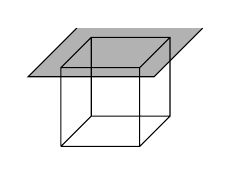
\begin{tikzpicture}
                    % Cube
                    \draw[-]
                       (0,0,0)
                    -- (1,0,0)
                    -- (1,1,0)
                    -- (0,1,0)
                    -- (0,0,0)
                       (0,0,1)
                    -- (1,0,1)
                    -- (1,1,1)
                    -- (0,1,1)
                    -- (0,0,1)
                    (0,0,0) -- (0,0,1)
                    (0,1,0) -- (0,1,1)
                    (1,1,0) -- (1,1,1)
                    (1,0,0) -- (1,0,1);
                    % Plano (001)
                    \draw[-, fill, fill opacity=0.3]
                       (1+0.3, 1, 0-0.3)
                    -- (1+0.3, 1, 1+0.3)
                    -- (0-0.3, 1, 1+0.3)
                    -- (0-0.3, 1, 0-0.3);
                    
                \end{tikzpicture}
            \end{questionBox}
    
            \begin{questionBox}3b{ % Q4.1.2
                \((1\,1\,0)\)
            } % Q4.1.2
                % \tikzset{external/remake next=true}
                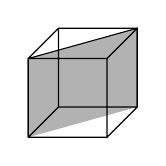
\begin{tikzpicture}
                    % Cube
                    \draw[-]
                       (0,0,0)
                    -- (1,0,0)
                    -- (1,1,0)
                    -- (0,1,0)
                    -- (0,0,0)
                       (0,0,1)
                    -- (1,0,1)
                    -- (1,1,1)
                    -- (0,1,1)
                    -- (0,0,1)
                    (0,0,0) -- (0,0,1)
                    (0,1,0) -- (0,1,1)
                    (1,1,0) -- (1,1,1)
                    (1,0,0) -- (1,0,1);
                    % Plano (110)
                    \draw[-, fill, fill opacity=0.3]
                       (0,0,1)
                    -- (0,1,1)
                    -- (1,1,0)
                    -- (1,0,0);
                \end{tikzpicture}
            \end{questionBox}
            \begin{questionBox}3b{ % Q4.1.3
                \((1\,1\,1)\)
            } % Q4.1.2
                % \tikzset{external/remake next=true}
                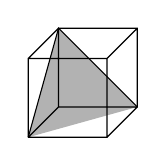
\begin{tikzpicture}
                    % Cube
                    \draw[-]
                       (0,0,0)
                    -- (1,0,0)
                    -- (1,1,0)
                    -- (0,1,0)
                    -- (0,0,0)
                       (0,0,1)
                    -- (1,0,1)
                    -- (1,1,1)
                    -- (0,1,1)
                    -- (0,0,1)
                    (0,0,0) -- (0,0,1)
                    (0,1,0) -- (0,1,1)
                    (1,1,0) -- (1,1,1)
                    (1,0,0) -- (1,0,1);
                    % Plano (111)
                    \draw[-, fill, fill opacity=0.3]
                       (1,0,0)
                    -- (0,1,0)
                    -- (0,0,1);
                \end{tikzpicture}
            \end{questionBox}
        \end{multicols}
    \end{questionBox}
    \begin{questionBox}2{ % Q4.2
        Sobre os planos anteriores desenhe, respectivamente, as direções:
        \begin{enumerate}[label={\roman{enumi}:}]
            \begin{multicols}{3}
                \item \([2\,1\,0]\)
                \item \([\bar{1}\,1\,1]\)
                \item \([1\,0\,\bar{1}]\)
            \end{multicols}
        \end{enumerate}
    } % Q4.2
        \answer{}
        \begin{multicols}{3}
            \begin{questionBox}3b{ % Q4.2.1
                \([2\,1\,0]\)
            } % Q4.2.1
                % \tikzset{external/remake next=true}
                \begin{tikzpicture}
                    % Cube
                    \draw[-]
                    (0,0,0)
                    -- (1,0,0)
                    -- (1,1,0)
                    -- (0,1,0)
                    -- (0,0,0)
                    (0,0,1)
                    -- (1,0,1)
                    -- (1,1,1)
                    -- (0,1,1)
                    -- (0,0,1)
                    (0,0,0) -- (0,0,1)
                    (0,1,0) -- (0,1,1)
                    (1,1,0) -- (1,1,1)
                    (1,0,0) -- (1,0,1);
                    % Plano (001)
                    \draw[-, fill, fill opacity=0.3]
                    (1+0.3, 1, 0-0.3)
                    -- (1+0.3, 1, 1+0.3)
                    -- (0-0.3, 1, 1+0.3)
                    -- (0-0.3, 1, 0-0.3);
                    % Direção [210]
                    \draw[->,Graph, thick]
                    (0,1,0) -- (.5,1,1);
                    
                \end{tikzpicture}
            \end{questionBox}

            \begin{questionBox}3b{ % Q4.1.2
                \([\bar{1}\,1\,1]\)
            } % Q4.1.2
                % \tikzset{external/remake next=true}
                \begin{tikzpicture}
                    % Cube
                    \draw[-]
                    (0,0,0)
                    -- (1,0,0)
                    -- (1,1,0)
                    -- (0,1,0)
                    -- (0,0,0)
                    (0,0,1)
                    -- (1,0,1)
                    -- (1,1,1)
                    -- (0,1,1)
                    -- (0,0,1)
                    (0,0,0) -- (0,0,1)
                    (0,1,0) -- (0,1,1)
                    (1,1,0) -- (1,1,1)
                    (1,0,0) -- (1,0,1);
                    % Plano (110)
                    \draw[-, fill, fill opacity=0.3]
                    (0,0,1)
                    -- (0,1,1)
                    -- (1,1,0)
                    -- (1,0,0);
                    % Direção [-111]
                    \draw[->,Graph,thick]
                    (0,0,1) -- (1,1,0);
                \end{tikzpicture}
            \end{questionBox}
            \begin{questionBox}3b{ % Q4.1.3
                \([1\,0\,\bar{1}]\)
            } % Q4.1.2
                % \tikzset{external/remake next=true}
                \begin{tikzpicture}
                    % Cube
                    \draw[-]
                    (0,0,0)
                    -- (1,0,0)
                    -- (1,1,0)
                    -- (0,1,0)
                    -- (0,0,0)
                    (0,0,1)
                    -- (1,0,1)
                    -- (1,1,1)
                    -- (0,1,1)
                    -- (0,0,1)
                    (0,0,0) -- (0,0,1)
                    (0,1,0) -- (0,1,1)
                    (1,1,0) -- (1,1,1)
                    (1,0,0) -- (1,0,1);
                    % Plano (111)
                    \draw[-, fill, fill opacity=0.3]
                       (1,0,0)
                    -- (0,1,0)
                    -- (0,0,1);
                    \draw[->,Graph,thick]
                    (0,1,0) -- (0,0,1);
                \end{tikzpicture}
            \end{questionBox}
        \end{multicols}
    \end{questionBox}
\end{questionBox}

\begin{questionBox}1{ % Q5
    O \ch{Pb} possui estrutura Cúbica de Faces Centradas (CFC) e o seu parâmetro de rede é \(a_{\ch{Pb}}=4.95\,\si{\angstrom}\). Quantos átomos por \si{\milli\metre^2} existem nos planos (1\,0\,0) e (1\,1\,1) do chumbo?
} % Q5
    \answer{}
    \begin{flalign*}
        &
            \text{(100)}:&\\&
            \frac{N_{atomos}}{\text{Area}}
            = \frac{2}{a^2}
            = \frac{2}{(4.95\E-7)^2}
            \cong 
            \SI{8.1624324048566e12}{Atomos/\milli\metre^2}
            ;&\\[3ex]&
            \text{(111)}:&\\&
            \frac{N_{atomos}}{\text{Area}}
            = \frac{3*1/2+3*1/6}{a\,\sqrt{2}*a\,\sqrt{2}\,\sin(\pi/3)/2}
            = \frac{4}{(4.95\E-7)^2\,\sqrt{3}}
            \cong &\\&
            \cong\SI{9.42516509237222e12}{Atomo/\milli\metre^2}
        &
    \end{flalign*}
\end{questionBox}

\begin{questionBox}1{ % Q6
    O cobre tem uma estrutura CFC e um raio atómico de 1.278\,\si{\angstrom}. Quantas camadas de planos \{1\,0\,0\} existem ao longo da espessura de uma película de 1\,\si{\micro\metre} de espessura. Suponha que os planos (0\,0\,1) são paralelos às superfícies superior e inferior da película.
} % Q6
    \answer{}
    \begin{flalign*}
        &
            \left\lfloor
                \frac{1\,\si{\micro\metre}}{a}
            \right\rfloor
            = \left\lfloor
                \frac{1\,\si{\micro\metre}}{r\,2^{3/2}}
            \right\rfloor
            = \left\lfloor
                \frac{1\,\si{\micro\metre}}{
                    (1.278\E-4)
                    \,2^{3/2}
                }
            \right\rfloor
            = 2766
        &
    \end{flalign*}
\end{questionBox}

\end{document}